%  Preprints.org version of the SankeyQA study, in the MDPI LaTeX template (version of September 2026) with the
%  journal option "preprints". Built by build_preprints.py, which fills the tables, the robustness paragraph and the
%  references and writes main.tex. Edit this file, not main.tex.

%=================================================================
\documentclass[preprints,article,accept,moreauthors]{Definitions/mdpi}

%=================================================================
% MDPI internal commands - do not modify
\firstpage{1}
\makeatletter
\setcounter{page}{\@firstpage}
\makeatother
\pubvolume{1}
\issuenum{1}
\articlenumber{0}
\pubyear{2026}
\copyrightyear{2026}
\datereceived{ }
\daterevised{ }
\dateaccepted{ }
\datepublished{ }

%=================================================================
\Title{Can Small Vision-Language Models Explain Career Maps? Reading the Picture or the Data behind a Sankey Diagram}


\newcommand{\orcidauthorA}{0000-0001-6727-1014}

\Author{Nikolaos~D.~Tantaroudas~$^{1,}$*\orcidA{}, Andrew~J.~McCracken~$^{2}$, Ilias~Karachalios~$^{3}$ and Evangelos~Papatheou~$^{4}$}

\AuthorNames{Nikolaos D. Tantaroudas, Andrew J. McCracken, Ilias Karachalios and Evangelos Papatheou}


\address{%
$^{1}$ \quad Institute of Communication and Computer Systems (ICCS), National Technical University of Athens, Iroon Polytechneiou 9, 15773 Zografou, Athens, Greece\\
$^{2}$ \quad DASKALOS-APPS, 183 Rue de l'Abb\'{e} Griffon, 01960 P\'{e}ronnas, France\\
$^{3}$ \quad University of Thessaly, 413 34 Larissa, Greece\\
$^{4}$ \quad Exeter Small-Scale Robotics Laboratory, Engineering Department, University of Exeter, Exeter EX4 4QF, United Kingdom}

\corres{Correspondence: nikolaos.tantaroudas@iccs.gr}

\abstract{Career guidance platforms such as XR-CareerAssist show possible careers as Sankey diagrams, in which bands of varying width show how many people moved between roles or industries over 2, 5 and 10 years. A virtual assistant that explains such a map can read the picture with a vision-language model or read the table of numbers behind it. This paper compares the two on SankeyQA, a new open benchmark of 600 artificial career maps with 6,560 questions whose answers are computed exactly from the underlying tables. The data are not real, they were generated by a computer only to demonstrate and test the technology, and no personal data are used. Five small open models that run on a laptop processor answered 875 questions about 80 unseen maps. A direct look-up in the table was always right. The best picture reader, SmolVLM-500M, answered 30.1\% of the questions correctly and a small language model reading the table 38.9\%, while a guess that never looks at the map reached 40.5\%. The picture readers could not read the numbers printed in the maps and rarely followed flows correctly. Fine-tuning BLIP on 400 maps raised its accuracy from 12.7\% to 55.5\%, and 20 maps chosen for diversity by k-means were no better than 20 random maps. An assistant that explains career maps should therefore answer from the data and use the picture to show the answer. The benchmark, the code and all model replies are openly available.}

\keyword{Sankey diagram, vision-language model, chart question answering, career guidance, extended reality, benchmark, fine-tuning, synthetic data}

%=================================================================
\begin{document}

\section{Introduction}

Career guidance tools increasingly show people pictures of possible futures. A common picture is the Sankey diagram, in which coloured bands flow from left to right and the width of each band shows how many people moved from one role, or one industry, to another~\cite{schmidt2008,riehmann2005}. The XR-CareerAssist platform places such career maps inside a virtual reality headset~\cite{tantaroudas2026salento,tantaroudas2026ore,tantaroudas2026arxiv}. A user answers a short questionnaire, the platform finds professionals with similar profiles in a database of more than 100,000 anonymised CVs, and a 3D avatar explains where these people were 2, 5 and 10 years later.

Sankey diagrams are compact but hard to read. Readers must compare the widths of curved bands, which people judge less accurately than positions or lengths~\cite{cleveland1984}, and the bands cross when groups exchange members~\cite{zarate2018}. Career guidance theory asks for exploration and dialogue rather than a single recommendation~\cite{savickas2012,leung2022}, so a career map needs a guide that answers questions about it correctly. In the XR-CareerAssist project, a fine-tuned BLIP vision-language model~\cite{li2022blip} was tried for this role. Training on 1,280 near-identical maps made it memorise them, 20 maps chosen by k-means gave better answers, and in the end a conversational agent that did not look at the picture guided the users~\cite{tantaroudas2026ore}. None of this could be measured, because there were no questions with known answers.

Because a Sankey diagram is drawn from a table of counts, every question about it has an exact answer that can be computed from the table. Chart question answering benchmarks use this idea for bar, line and pie charts~\cite{kahou2018,kafle2018,methani2020,masry2022}, but, as far as the authors know, not for Sankey diagrams. This paper builds such a benchmark for career maps and asks whether small models that run on a laptop can read the picture, whether fine-tuning helps and whether diverse training maps help more than random ones, and whether an assistant should read the picture or the data. A full report of the study, with all tables, is in preparation for Open Research Europe.

\section{Materials and Methods}

\subsection{Benchmark}

Figure~\ref{fig:pipeline} shows the pipeline. Each questionnaire configuration (kind of map, starting role, years of experience, industry, age group, target role and 60 to 1,200 matched profiles) produces a simulated cohort, in which a small random model moves people between six ladder roles and two side roles, or between twelve industries, at 2, 5 and 10 years. As in the platform, each stage shows its four to seven largest groups and merges the rest into Other. The cohort is summarised in a flow table, drawn as a career map with Matplotlib~\cite{hunter2007} (Figure~\ref{fig:example}), and used to generate eleven kinds of questions with exact answers, from the largest group at a stage to the size of a flow or the destination reached by following the main moves. The data are artificial and not real. They were generated only to demonstrate and test the technology, they contain no personal data, and they say nothing about real careers.

\begin{figure}[H]
\isPreprints{\centering}{}
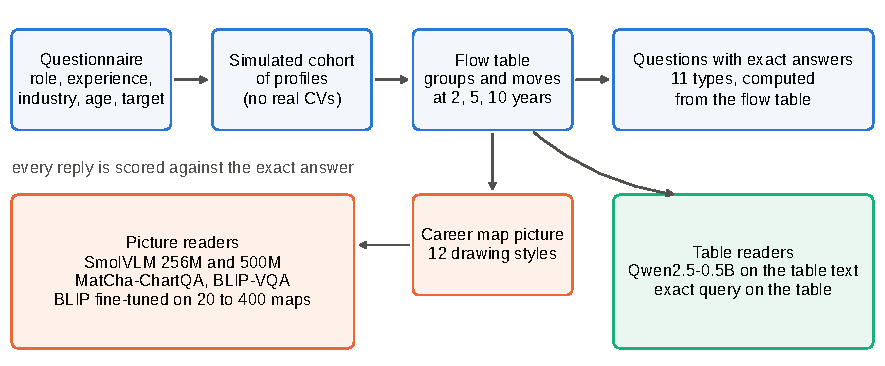
\includegraphics[width=\textwidth]{figures/fig1_pipeline.pdf}
\caption{How SankeyQA is built and used. A questionnaire configuration produces a simulated cohort, whose flow table gives both the drawn career map and questions with exact answers. Picture readers see only the map, table readers only the flow table.\label{fig:pipeline}}
\end{figure}

\begin{figure}[H]
\isPreprints{\centering}{}
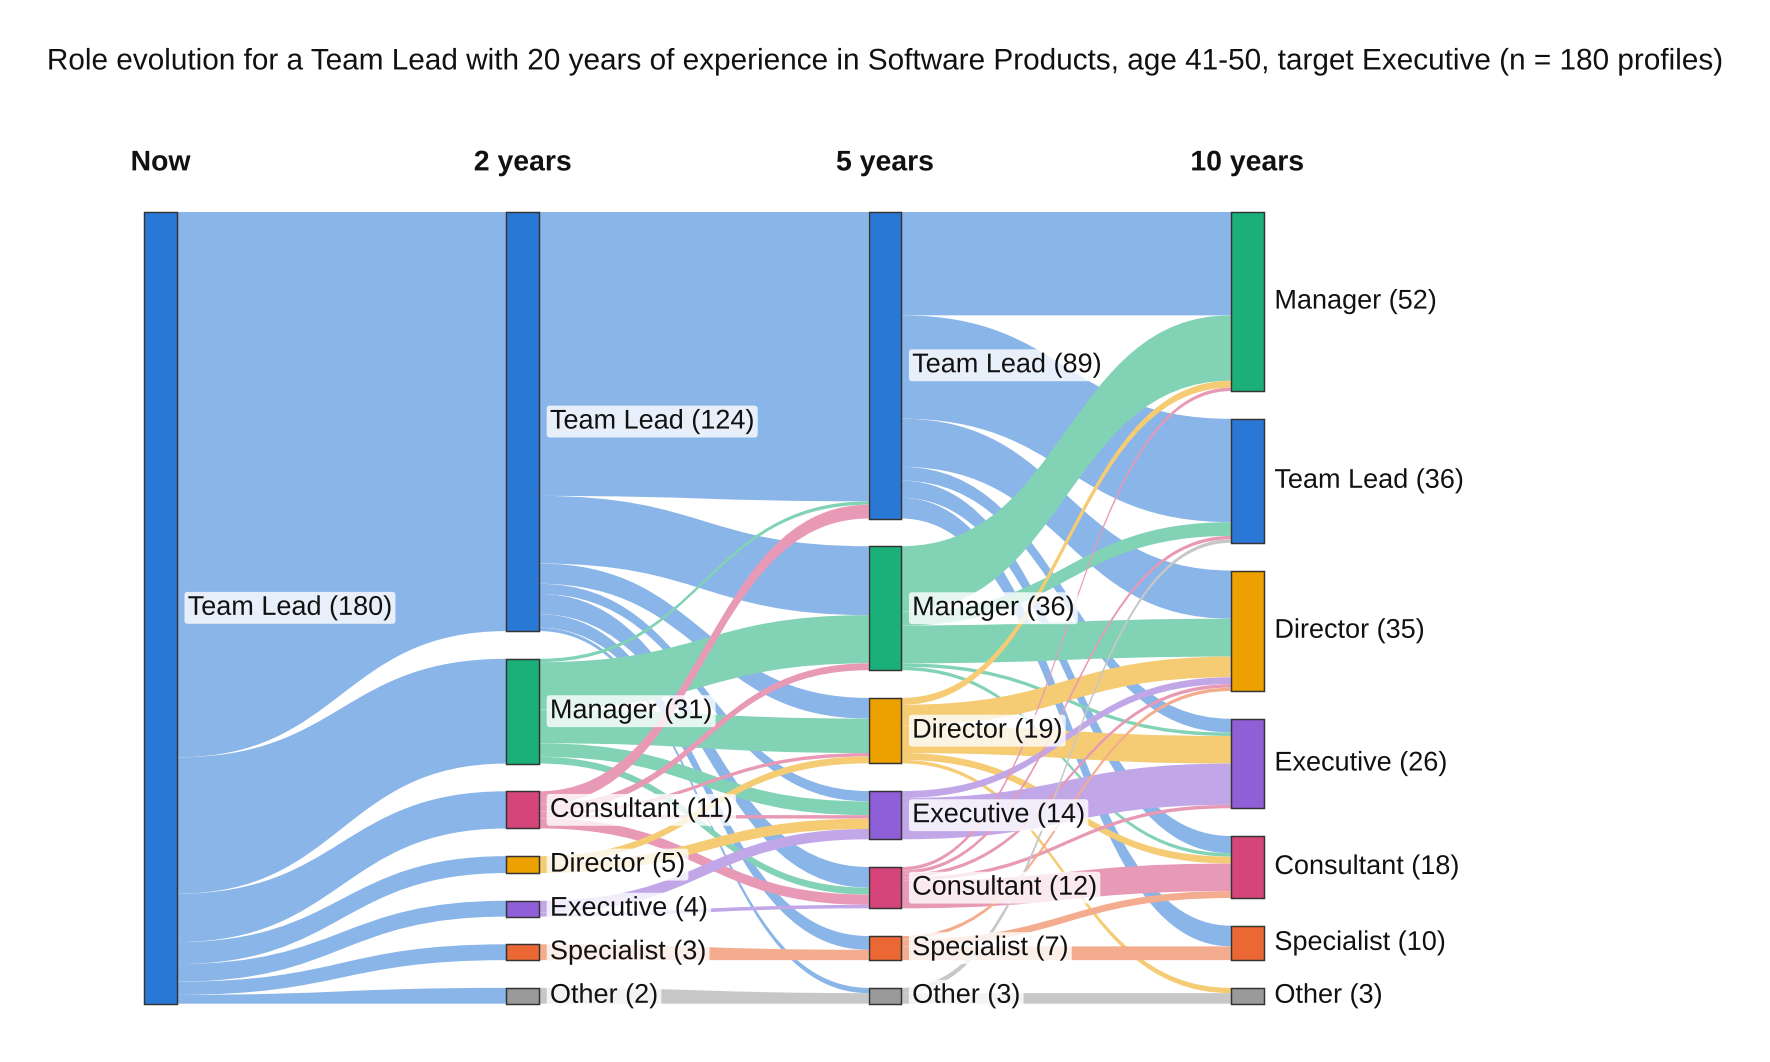
\includegraphics[width=0.92\textwidth]{figures/fig2_role_example.png}
\caption{A role map of the test split in the default style. Bars are groups of profiles at each stage, with their size in brackets, and the width of a band is the number of profiles moving between two groups.\label{fig:example}}
\end{figure}

The benchmark has 600 cohorts (358 role maps, 242 industry maps) and 6,560 questions. The first 400 cohorts are used for training and the last 200 for testing. The main evaluation uses 80 test maps (875 questions). Twenty test maps were also drawn in eleven other styles, each changing one setting such as a transparent background, no numbers, larger or smaller text, one colour or a lower resolution (220 questions per style).

\subsection{Readers and scoring}

The picture readers were SmolVLM-256M and SmolVLM-500M~\cite{marafioti2025}, MatCha-ChartQA~\cite{liu2023matcha,lee2023pix2struct} and BLIP-VQA~\cite{li2022blip}. The table readers were Qwen2.5-0.5B-Instruct~\cite{qwen2025}, which received the flow table as text, and an exact query on the table. Two baselines needed no reading, a random choice among the possible answers and a guess that never looks at the map (the starting role or industry for name questions, the most common or median training answer otherwise). All models ran with the Transformers library~\cite{wolf2020} on two processor cores with greedy decoding. Numbers counted as correct within 5\% or one unit, as in chart benchmarks~\cite{methani2020,masry2022}, and 95\% intervals come from 2,000 bootstrap resamples of maps~\cite{efron1979}.

BLIP-VQA was also fine-tuned, with its image encoder fixed, for 600 updates of 8 questions with AdamW~\cite{loshchilov2019}. The training maps were 20 diverse maps, the map nearest to each of 20 k-means clusters of image features~\cite{lloyd1982,sener2018}, or 20 (three draws), 100 or 400 random maps. Every run thus had the same budget and differed only in its training maps.

\section{Results}

Table~\ref{tab:overall} shows the main result. The exact query answered every question correctly. The best picture reader answered 30.1\% correctly and the table reader 38.9\%, while the guess reached 40.5\%. MatCha-ChartQA and BLIP-VQA often replied with something that was not an answer, such as a position in the picture, and scored below random choice.

{{TAB_OVERALL}}

Figure~\ref{fig:qtype} breaks the results down. The picture readers almost never read the numbers printed in the map, so the total and the sizes of groups were rarely right, while the table reader copied the total from its table every time. Questions that need only a comparison of sizes went better, but following the main moves over several stages was right in at most 28.0\% of cases for any model before fine-tuning. The guess did well wherever the answer follows the typical shape of the maps, which shows that such a baseline must be reported.

\begin{figure}[H]
\isPreprints{\centering}{}
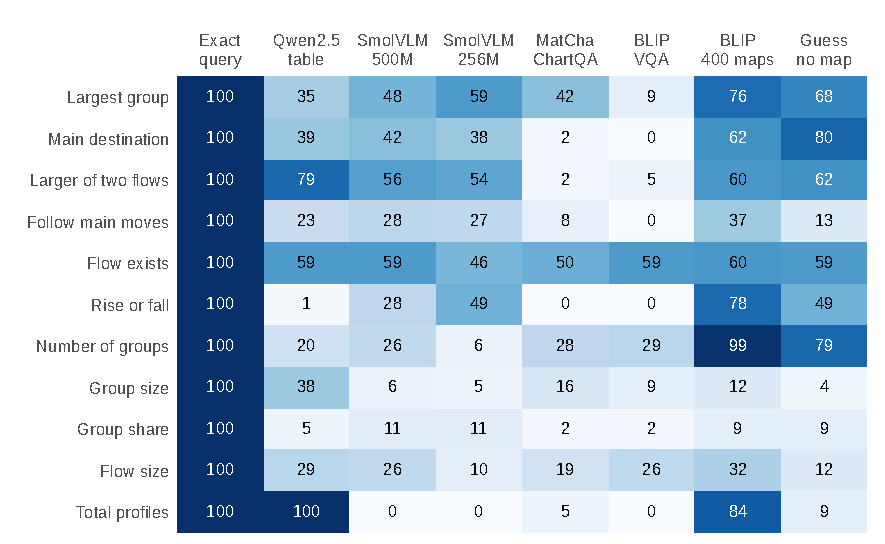
\includegraphics[width=\textwidth]{figures/fig3_accuracy_by_question.pdf}
\caption{Correct answers (\%) by kind of question (rows) and reader (columns) on the 875 test questions. BLIP 400 maps is BLIP-VQA after fine-tuning on 400 maps.\label{fig:qtype}}
\end{figure}

{{ROBUST_SHORT}}

Fine-tuning raised BLIP-VQA from 12.7\% to between 43.9\% and 55.5\% (Table~\ref{tab:ft}). The 20 diverse maps gave 45.3\%, within the range of the three random draws of 20 maps. The diverse maps did better on name questions and worse on number questions. More maps helped more, 54.2\% with 100 maps and 55.5\% with 400 maps.

{{TAB_FT}}

\section{Discussion and Conclusions}

When an application has the table that a chart was drawn from, it should answer from the table. A direct look-up was always right and took less than a millisecond, while every small model, including a language model given the same table, was wrong most of the time. This confirms with measurements the design decision of XR-CareerAssist, whose conversational agent rather than its vision-language model guided users through the maps~\cite{tantaroudas2026ore}. An assistant can pass the user's question to a few look-up functions and let a language model only phrase the answer, while the picture shows the user the shape of the possible careers.

The picture readers failed for three reasons. They could not read small printed numbers at their input resolution, Sankey diagrams encode quantities in band widths that are hard to compare~\cite{cleveland1984}, and the chart model was trained on other kinds of charts~\cite{masry2022} and often produced text that was not an answer, a known weakness of vision-language models~\cite{li2023hallucination}. Fine-tuning made the task learnable but did not solve it. The project's observation that 20 diverse maps beat 1,280 maps is best explained by the near-duplicates in its data, because with varied maps a careful choice of 20 was no better than chance and more maps helped more.

The maps are artificial, generated only to test the technology, the models are small, each received one instruction and only BLIP was fine-tuned, and these limits are discussed in the full report. Larger models and real maps can be added with the same code. SankeyQA, its generator and all replies are openly available for testing future models.

%%%%%%%%%%%%%%%%%%%%%%%%%%%%%%%%%%%%%%%%%%
\vspace{6pt}

\funding{This work was supported by the European Union's Horizon Europe research and innovation programme through Financial Support to Third Parties of the VOXReality project, Voice driven interaction in XR spaces (Grant Agreement No.\ 101070521). Views and opinions expressed are those of the authors only and do not necessarily reflect those of the European Union or the granting authority. Neither the European Union nor the granting authority can be held responsible for them.}

\institutionalreview{Not applicable, the study involved no human participants and no personal data.}

\informedconsent{Not applicable.}

\dataavailability{The benchmark (flow tables, 1,260 images and 6,560 questions), every model reply, all result tables and the code that generates the benchmark, runs the models and draws the figures are available on GitHub at \url{ {{GITHUB_SHORT}} } and archived on Zenodo~\cite{sankeyqadata}, under the Apache 2.0 licence for the code and CC BY 4.0 for the data.}

\acknowledgments{The authors thank the VOXReality consortium for the support given to XR-CareerAssist. During the preparation of this work the authors used an AI assistant (Claude, Anthropic) to help write the code and draft the text. The authors reviewed and edited all code and text and take full responsibility for the content.}

\conflictsofinterest{The authors developed the XR-CareerAssist platform. N.D.T. is the founder of DASKALOS APPS SAS, with which A.J.M. is affiliated. The authors declare no other conflicts of interest.}

%%%%%%%%%%%%%%%%%%%%%%%%%%%%%%%%%%%%%%%%%%
\reftitle{References}

{{BIB}}

\PublishersNote{}
\end{document}
